% Options for packages loaded elsewhere
\PassOptionsToPackage{unicode}{hyperref}
\PassOptionsToPackage{hyphens}{url}
\PassOptionsToPackage{dvipsnames,svgnames,x11names}{xcolor}
%
\documentclass[12pt, oneside]{report}

% Inputs the Document Packages
\usepackage{array}
\usepackage{blindtext}
\usepackage[
    citestyle=verbose-ibid,
    bibstyle=authoryear,
    autocite=footnote,
    notetype=endonly,
    backend=biber,
    isbn=false, 
    doi=false,
    labeldateparts
]{biblatex}
\usepackage{booktabs}
\usepackage{ctable}
\usepackage{fancyhdr}
\usepackage{graphicx}
\usepackage[hidelinks]{hyperref}
\usepackage[utf8]{inputenc}
\usepackage{mobilizing-justice}
\usepackage{multicol}
\usepackage{pdfpages}
% Change font size
\usepackage{relsize}
\usepackage{setspace}
\usepackage{subfig}
\usepackage{tcolorbox}
\tcbuselibrary{theorems}
\usepackage{wrapfig}


% Pointing to a bib resource here
\addbibresource[label=main]{bibliography.bib} % REPLACE WITH WORKS CITED BIB FILE

% Remove URL and DOI for cleaner citations (optional, obviously)
\AtEveryBibitem{
    \clearfield{url}
    \clearfield{doi}
}

\let\oldheadrule\headrule% Copy \headrule into \oldheadrule
\renewcommand{\headrule}{\color{Maroon}\oldheadrule}% Add colour to \headrule
\renewcommand{\headrulewidth}{12.5pt}

% HERE GOES THE RUNNING TITLE FOR THE FOOTER
\title{Mobilizing Justice Report}

%-------------------------Header & Footer------------------------

% PAGESTYLE FANCY IS THE DEFAULT
\pagestyle{fancy}
\fancyhf{}
\renewcommand{\footrulewidth}{0pt}
\fancyfoot[R]{\textbf{\thepage}}
\fancyfoot[L]{\nouppercase\@title} % HERE GOES THE TITLE
\renewcommand{\footrulewidth}{1pt}

% PAGESTYLE plain (IS IT EVEN USED?)
\fancypagestyle{plain}{%
  \renewcommand{\headrulewidth}{0pt}%
  \fancyhf{}%
  \renewcommand{\footrulewidth}{1pt}
  \fancyfoot[R]{\textbf{\thepage}}%
  \fancyfoot[L]{\nouppercase\@title} % HERE GOES THE TITLE
}

% PAGESTYLE title-page (IS IT EVEN USED?)
\fancypagestyle{title-page}{%
  \renewcommand{\headrulewidth}{0pt}%
  \fancyhf{}%
  \renewcommand{\footrulewidth}{0pt}
}

\usepackage{amsmath,amssymb}
\usepackage{iftex}
\ifPDFTeX
  \usepackage[T1]{fontenc}
  \usepackage[utf8]{inputenc}
  \usepackage{textcomp} % provide euro and other symbols
\else % if luatex or xetex
  \usepackage{unicode-math}
  \defaultfontfeatures{Scale=MatchLowercase}
  \defaultfontfeatures[\rmfamily]{Ligatures=TeX,Scale=1}
\fi
\usepackage{lmodern}
\ifPDFTeX\else  
    % xetex/luatex font selection
\fi
% Use upquote if available, for straight quotes in verbatim environments
\IfFileExists{upquote.sty}{\usepackage{upquote}}{}
\IfFileExists{microtype.sty}{% use microtype if available
  \usepackage[]{microtype}
  \UseMicrotypeSet[protrusion]{basicmath} % disable protrusion for tt fonts
}{}
\makeatletter
\@ifundefined{KOMAClassName}{% if non-KOMA class
  \IfFileExists{parskip.sty}{%
    \usepackage{parskip}
  }{% else
    \setlength{\parindent}{0pt}
    \setlength{\parskip}{6pt plus 2pt minus 1pt}}
}{% if KOMA class
  \KOMAoptions{parskip=half}}
\makeatother
\usepackage{xcolor}
\setlength{\emergencystretch}{3em} % prevent overfull lines
\setcounter{secnumdepth}{-\maxdimen} % remove section numbering
% Make \paragraph and \subparagraph free-standing
\ifx\paragraph\undefined\else
  \let\oldparagraph\paragraph
  \renewcommand{\paragraph}[1]{\oldparagraph{#1}\mbox{}}
\fi
\ifx\subparagraph\undefined\else
  \let\oldsubparagraph\subparagraph
  \renewcommand{\subparagraph}[1]{\oldsubparagraph{#1}\mbox{}}
\fi


\providecommand{\tightlist}{%
  \setlength{\itemsep}{0pt}\setlength{\parskip}{0pt}}\usepackage{longtable,booktabs,array}
\usepackage{calc} % for calculating minipage widths
% Correct order of tables after \paragraph or \subparagraph
\usepackage{etoolbox}
\makeatletter
\patchcmd\longtable{\par}{\if@noskipsec\mbox{}\fi\par}{}{}
\makeatother
% Allow footnotes in longtable head/foot
\IfFileExists{footnotehyper.sty}{\usepackage{footnotehyper}}{\usepackage{footnote}}
\makesavenoteenv{longtable}
\usepackage{graphicx}
\makeatletter
\def\maxwidth{\ifdim\Gin@nat@width>\linewidth\linewidth\else\Gin@nat@width\fi}
\def\maxheight{\ifdim\Gin@nat@height>\textheight\textheight\else\Gin@nat@height\fi}
\makeatother
% Scale images if necessary, so that they will not overflow the page
% margins by default, and it is still possible to overwrite the defaults
% using explicit options in \includegraphics[width, height, ...]{}
\setkeys{Gin}{width=\maxwidth,height=\maxheight,keepaspectratio}
% Set default figure placement to htbp
\makeatletter
\def\fps@figure{htbp}
\makeatother
\newlength{\cslhangindent}
\setlength{\cslhangindent}{1.5em}
\newlength{\csllabelwidth}
\setlength{\csllabelwidth}{3em}
\newlength{\cslentryspacingunit} % times entry-spacing
\setlength{\cslentryspacingunit}{\parskip}
\newenvironment{CSLReferences}[2] % #1 hanging-ident, #2 entry spacing
 {% don't indent paragraphs
  \setlength{\parindent}{0pt}
  % turn on hanging indent if param 1 is 1
  \ifodd #1
  \let\oldpar\par
  \def\par{\hangindent=\cslhangindent\oldpar}
  \fi
  % set entry spacing
  \setlength{\parskip}{#2\cslentryspacingunit}
 }%
 {}
\usepackage{calc}
\newcommand{\CSLBlock}[1]{#1\hfill\break}
\newcommand{\CSLLeftMargin}[1]{\parbox[t]{\csllabelwidth}{#1}}
\newcommand{\CSLRightInline}[1]{\parbox[t]{\linewidth - \csllabelwidth}{#1}\break}
\newcommand{\CSLIndent}[1]{\hspace{\cslhangindent}#1}

% TODO: Add custom LaTeX header directives here
\makeatletter
\makeatother
\makeatletter
\makeatother
\makeatletter
\@ifpackageloaded{caption}{}{\usepackage{caption}}
\AtBeginDocument{%
\ifdefined\contentsname
  \renewcommand*\contentsname{Table of contents}
\else
  \newcommand\contentsname{Table of contents}
\fi
\ifdefined\listfigurename
  \renewcommand*\listfigurename{List of Figures}
\else
  \newcommand\listfigurename{List of Figures}
\fi
\ifdefined\listtablename
  \renewcommand*\listtablename{List of Tables}
\else
  \newcommand\listtablename{List of Tables}
\fi
\ifdefined\figurename
  \renewcommand*\figurename{Figure}
\else
  \newcommand\figurename{Figure}
\fi
\ifdefined\tablename
  \renewcommand*\tablename{Table}
\else
  \newcommand\tablename{Table}
\fi
}
\@ifpackageloaded{float}{}{\usepackage{float}}
\floatstyle{ruled}
\@ifundefined{c@chapter}{\newfloat{codelisting}{h}{lop}}{\newfloat{codelisting}{h}{lop}[chapter]}
\floatname{codelisting}{Listing}
\newcommand*\listoflistings{\listof{codelisting}{List of Listings}}
\makeatother
\makeatletter
\@ifpackageloaded{caption}{}{\usepackage{caption}}
\@ifpackageloaded{subcaption}{}{\usepackage{subcaption}}
\makeatother
\makeatletter
\@ifpackageloaded{tcolorbox}{}{\usepackage[skins,breakable]{tcolorbox}}
\makeatother
\makeatletter
\@ifundefined{shadecolor}{\definecolor{shadecolor}{rgb}{.97, .97, .97}}
\makeatother
\makeatletter
\makeatother
\makeatletter
\makeatother
\ifLuaTeX
  \usepackage{selnolig}  % disable illegal ligatures
\fi
\IfFileExists{bookmark.sty}{\usepackage{bookmark}}{\usepackage{hyperref}}
\IfFileExists{xurl.sty}{\usepackage{xurl}}{} % add URL line breaks if available
\urlstyle{same} % disable monospaced font for URLs
\hypersetup{
  pdftitle={Mobilizing Justice Report},
  pdfauthor={Author One; Author Two},
  colorlinks=true,
  linkcolor={blue},
  filecolor={Maroon},
  citecolor={Blue},
  urlcolor={Blue},
  pdfcreator={LaTeX via pandoc}}

\title{Mobilizing Justice Report}
\author{Author One \and Author Two}
\date{2023-11-11}

\begin{document}
%
%
%

% START OF TITLE PAGE
\thispagestyle{empty}

% Define a dimension for the height of the banner for the title page
\newdimen\bannerheight

% Set \bannerheight to the height of the banner
\settoheight{\bannerheight}{%
  
\includegraphics[width=\paperwidth]{images/title-banner.png}%
}

% Title banner top
\AddToShipoutPictureBG*{%
 \AtPageUpperLeft{\raisebox{-\height}{
\includegraphics[width=\paperwidth]{images/title-banner.png}}}
 }

% Cover picture
\AddToShipoutPictureBG*{%
 %\AtPageLowerLeft{\raisebox{0.5\height}{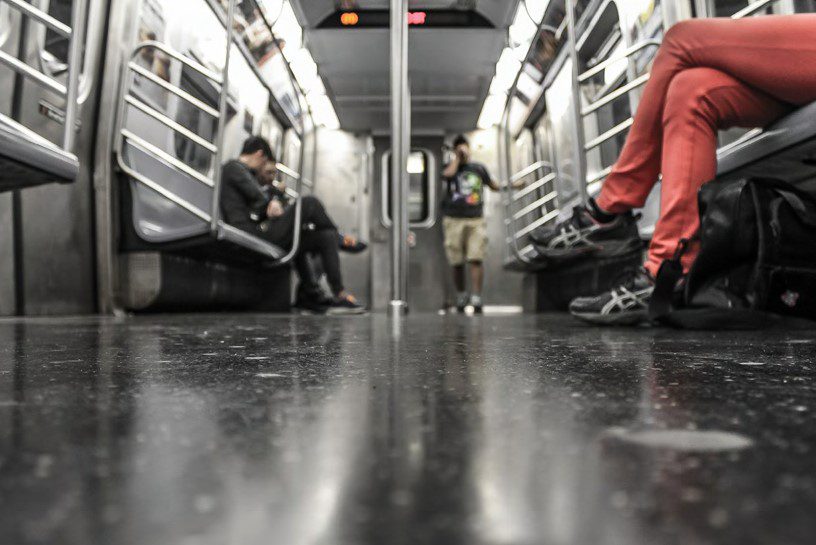
\includegraphics[width=\paperwidth]{images/cover-picture.png}}}
 \AtPageUpperLeft{\raisebox{-\bannerheight-\height}{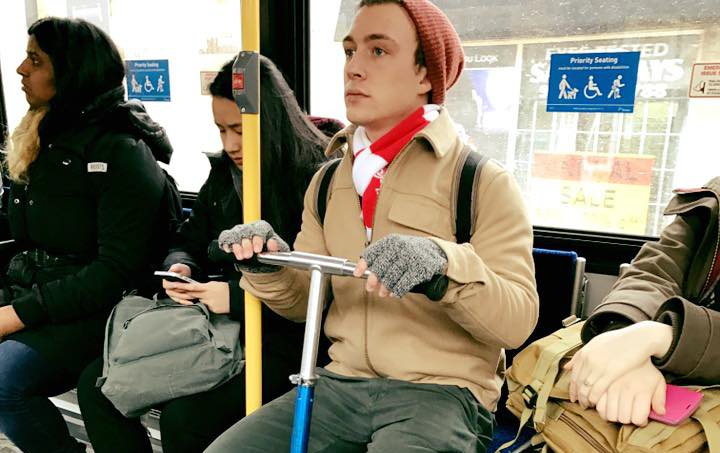
\includegraphics[width=\paperwidth]{images/cover-picture2.png}}}
 }

% Report information: Needs information that is in file template.qmd
\begin{flushleft}
    \vspace{-7cm}
              {\relscale{2}{\textcolor{white}{Mobilizing Justice
Report}}}\\ % HERE GOES THE TITLE OF THE DOCUMENT 
            \vspace{1cm} 
      
      % TODO: IT IS NOT PRINTING THE AFFILIATIONS CORRECTLY
              {\relscale{1.5}{\textcolor{Yellow}{Author
One}}}\hskip 10pt {Some affiliation}\par % HERE GO THE AUTHORS + POSSIBLY AFFILIATIONS (CURRENTLY NOT WORKING)
              {\relscale{1.5}{\textcolor{Yellow}{Author
Two}}}\hskip 10pt {Some affiliation}\par % HERE GO THE AUTHORS + POSSIBLY AFFILIATIONS (CURRENTLY NOT WORKING)
      \end{flushleft}

\begin{flushright}
    \vspace{-1cm}
        {\relscale{1.5}{\textcolor{Yellow}{Report}}}\\ % HERE GOES THE DOCUMENT TYPE; CURRENTLY HARDCODED BUT COULD BE AN INPUT IN template.qmd
        \vspace{1cm}     
        {\relscale{1.5}{\textcolor{LightGray}{2023-11-11}}} % HERE GOES THE DATE OF PUBLICATION
\end{flushright}

% Mobilizing Justice Logo
\AddToShipoutPictureBG*{\put(30,30)%
{
\includegraphics[width=0.5\textwidth]{images/mj-logo.png}%
}}

%\AddToShipoutPictureBG*{%
% \AtPageLowerLeft{\raisebox{\height}{
\includegraphics[width=0.5\textwidth]{images/mj-logo.png}}}
% }

% END OF TITLE PAGE

\newpage

% START OF ABOUT PAGE

\section*{About Mobilizing Justice}

The Mobilizing Justice Partnership is funded by the Social Sciences and Humanities Research Council (SSHRC). Based at the University of Toronto Scarborough, the national intersectoral research partnership aims to understand and address transportation poverty in Canada and to improve the well-being of Canadians at risk of transport poverty. Learn more at \url{www.mobilizingjustice.ca}.

% TABLE OF PARTNERS

\section*{Our Partners}
\begin{center}
\ctable[
%label = width,
width = \textwidth,
pos = ht,
left,
doinside = \relscale{0.87}{}
]{| >{\setlength{\baselineskip}{0.1\baselineskip}}>{\raggedright}X | >{\setlength{\baselineskip}{0.1\baselineskip}}>{\raggedright}X | >{\setlength{\baselineskip}{0.1\baselineskip}}>{\raggedright}X |}{}
{ \FL
Amalgamated Transit Union Canada                                                & Infrastructure Canada              & Transit App                                \LL
Autorité régionale de transport métropolitain (ARTM)                            & McGill University                  & TransLink                      \LL
Canadian Institute of Planners                                                  & McMaster University                & United   Way Greater Toronto   \LL
Canada Mortgage and Housing Corporation (CMHC)                                  & Memorial University                & University of British Columbia \LL
Canadian Urban Institute                                                        & Metrolinx                          & University of Manitoba         \LL
Canadian Urban Transit Association                                              & Ontario Ministry of Transportation & University of Oregon           \LL
The Centre for Active Transportation (TCAT), a project of Clean Air Partnership & Pantonium                          & University of Texas Austin     \LL
CIRODD (École de technologie supérieure)                                        & Pembina Institute                  & University of Toronto          \LL
CIRRELT (Université de Montréal)                                                & Region of Waterloo                 & University of Waterloo         \LL
City of Calgary                                                                 & RideShark                          & Urban Strategies               \LL
City of Edmonton                                                                & Simon Fraser University            & Via Transportation Inc.        \LL
City of Toronto                                                                 & Spare Labs                         & Ville de Montréal              \LL
City of Vancouver                                                               & SPIN                               & York Region                    \LL
Esri Canada                                                                     & Statistics Canada                  &    \LL
Federation of Canadian Municipalities	& Toronto Transit Commission (TTC)	& \LL
}
\end{center}

% END OF ABOUT PAGE

\newpage

% START OF TABLE OF CONTENTS PAGE

% Table of contents picture top
\AddToShipoutPictureBG*{%
 \AtPageUpperLeft{\raisebox{-\height}{\includegraphics[width=\paperwidth]{images/table-of-contents-picture.png}}}}

% Change the geometry of this one page so that the table of contents begins below the banner image instead of on top of it
\newgeometry{top=10cm}

% Title for the table of contents
%\renewcommand\contentsname{\color{DarkBlue}\normalfont\bfseries\fontsize{24}{28.8}\selectfont Table of Contents}
%\restoregeometry
%\newgeometry{left=5cm}
\setcounter{tocdepth}{1}
\tableofcontents
\restoregeometry

% ENDO OF TABLE OF CONTENTS

\newpage\ifdefined\Shaded\renewenvironment{Shaded}{\begin{tcolorbox}[interior hidden, enhanced, sharp corners, boxrule=0pt, frame hidden, borderline west={3pt}{0pt}{shadecolor}, breakable]}{\end{tcolorbox}}\fi

\hypertarget{introduction}{%
\section{Introduction}\label{introduction}}

\emph{TODO} Create an example file that demonstrates the formatting and
features of your format.

\hypertarget{more-information}{%
\section{More Information}\label{more-information}}

You can learn more about controlling the appearance of PDF output here:
\url{https://quarto.org/docs/output-formats/pdf-basics.html}

Here is an example of a reference: OECD (2013).

\newpage

\hypertarget{references}{%
\section{References}\label{references}}

\hypertarget{refs}{}
\begin{CSLReferences}{1}{0}
\leavevmode\vadjust pre{\hypertarget{ref-OECDFrameworks2013}{}}%
OECD. 2013. {``Frameworks and Sector Policies for Urban Development in
Chile.''} Book Section. In \emph{OECD Urban Policy Reviews, Chile 2013}.
https://doi.org/\url{http://dx.doi.org/10.1787/9789264191808-en}.

\end{CSLReferences}

\newpage

% LAST PAGE
% This page is left blank on purpose

% Set style for this page
\thispagestyle{empty}

% Council logo at bottom
\begin{center}
    \begin{figure}[b]
        
\includegraphics[width=\textwidth]{images/sshrc-canada-banner.png}
    \end{figure}    
\end{center}



\end{document}
